\documentclass[a4paper,10pt]{article}

\usepackage[brazilian]{babel}
\usepackage[left=2.5cm,right=2.5cm,top=3cm,bottom=2.5cm]{geometry}
\usepackage{mathtools}
\usepackage{amsthm}
\usepackage{amsmath}
%\usepackage{nccmath}
\usepackage{amssymb}
\usepackage{amsfonts}
\usepackage{physics}
%\usepackage{dsfont}
%\usepackage{mathrsfs}

\usepackage{titling}
\usepackage{indentfirst}

\usepackage{bm}
\usepackage[dvipsnames]{xcolor}
\usepackage{cancel}

\usepackage{xurl}
\usepackage[colorlinks=true]{hyperref}

\usepackage{float}
\usepackage{graphicx}
%\usepackage{tikz}
\usepackage{caption}
\usepackage{subcaption}

%%%%%%%%%%%%%%%%%%%%%%%%%%%%%%%%%%%%%%%%%%%%%%%%%%%

\newcommand{\eps}{\epsilon}
\newcommand{\vphi}{\varphi}
\newcommand{\cte}{\text{cte}}

\newcommand{\N}{\mathbb{N}}
\newcommand{\Z}{\mathbb{Z}}
\newcommand{\Q}{\mathbb{Q}}
\newcommand{\R}{\vb{R}}
\newcommand{\C}{\mathbb{C}}
\renewcommand{\S}{\hat{S}}
%\renewcommand{\H}{\s{H}}

\renewcommand{\a}{\vb{a}}
\newcommand{\nn}{\hat{n}}
\renewcommand{\d}{\dagger}
\newcommand{\up}{\uparrow}
\newcommand{\down}{\downarrow}

\newcommand{\0}{\vb{0}}
%\newcommand{\1}{\mathds{1}}
\newcommand{\E}{\vb{E}}
\newcommand{\B}{\vb{B}}
\renewcommand{\v}{\vb{v}}
\renewcommand{\r}{\vb{r}}
\renewcommand{\k}{\vb{k}}
\newcommand{\p}{\vb{p}}
\newcommand{\q}{\vb{q}}
\newcommand{\F}{\vb{F}}

\newcommand{\s}{\sigma}
%\newcommand{\prodint}[2]{\left\langle #1 , #2 \right\rangle}
\newcommand{\cc}[1]{\overline{#1}}
\newcommand{\Eval}[3]{\eval{\left( #1 \right)}_{#2}^{#3}}

\newcommand{\unit}[1]{\; \mathrm{#1}}

\newcommand{\n}{\medskip}
\newcommand{\e}{\quad \mathrm{e} \quad}
\newcommand{\ou}{\quad \mathrm{ou} \quad}
\newcommand{\virg}{\, , \;}
\newcommand{\ptodo}{\forall \,}
\renewcommand{\implies}{\; \Rightarrow \;}
%\newcommand{\eqname}[1]{\tag*{#1}} % Tag equation with name

\setlength{\droptitle}{-7em}

\theoremstyle{plain}
\newtheorem{theorem}{Teorema}[section]
%\newtheorem{defi}[theorem]{Definição}
\newtheorem{lemma}[theorem]{Lema}
%\newtheorem{corol}[theorem]{Corolário}
%\newtheorem{prop}[theorem]{Proposição}
%\newtheorem{example}{Exemplo}
%
%\newtheorem{inneraxiom}{Axioma}
%\newenvironment{axioma}[1]
%  {\renewcommand\theinneraxiom{#1}\inneraxiom}
%  {\endinneraxiom}
%
%\newtheorem{innerpostulado}{Postulado}
%\newenvironment{postulado}[1]
%  {\renewcommand\theinnerpostulado{#1}\innerpostulado}
%  {\endinnerpostulado}
%
%\newtheorem{innerexercise}{Exercício}
%\newenvironment{exercise}[1]
%  {\renewcommand\theinnerexercise{#1}\innerexercise}
%  {\endinnerexercise}
%
%\newtheorem{innerthm}{Teorema}
%\newenvironment{teorema}[1]
%  {\renewcommand\theinnerthm{#1}\innerthm}
%  {\endinnerthm}
%
\newtheorem{innerlema}{Lema}
\newenvironment{lema}[1]
  {\renewcommand\theinnerlema{#1}\innerlema}
  {\endinnerlema}
%
%\theoremstyle{remark}
%\newtheorem*{hint}{Dica}
%\newtheorem*{notation}{Notação}
%\newtheorem*{obs}{Observação}


\newcommand{\vac}{\ket{vac}}
\newcommand{\hh}{\tilde{h}}
\newcommand{\hhh}{\bm{\tilde{h}}}
\newcommand{\vecs}{(\s^x, \s^y, \s^z)}
\renewcommand{\ss}{\bm{\sigma}}


\title{\Huge{\textbf{Prova final - Mecânica Estatística}}}
\author{Mateus Marques}

\begin{document}

\maketitle

\section*{1) Modelo de Ising em um campo transverso}

(a) Primeiramente, observe que:
\begin{itemize}
\item Pelas relações de comutação de férmions, temos $[n_k, n_\ell] = 0$ para quaisquer sítios $k, \ell$.

\n

\item Em particular, a exponencial da soma $e^{\pm i\pi \sum_{k<j} n_k}$ pode ser separada no produto $\prod_{k<j} e^{\pm i\pi n_k}$, pois todos os operadores $n_k$ comutam entre si.

\n

\item Como $n_k^2 = n_k$ pelo princípio de Pauli, temos também $n_k^p = n_k$ para qualquer natural $p\geq 1$. Assim:
$$
e^{\pm i\pi n_k} = 1 + \sum_{p=1}^{\infty} \frac{(\pm i\pi n_k)^p}{p!} = 1+ \qty( \sum_{p=1}^{\infty} \frac{(\pm i\pi)^p}{p!} ) n_k = 1 + (e^{\pm i \pi} - 1) n_k = 1 - 2 n_k = - \s_j^z,
$$
$$
e^{\pm i\pi \sum_{k<j} n_k} = \prod_{k<j} e^{\pm i\pi n_k} = \prod_{k<j} (-\s_k^z).
$$

\end{itemize}

Temos então que
$$
\sigma_j^x = \frac{\qty(\sigma_j^+ + \sigma_j^-)}{2} =
e^{i\pi \sum_{k<j} n_k} f_j^\d + e^{-i\pi \sum_{k<j} n_k} f_j =
\qty[\prod_{k<j} (-\s_k^z)] \qty(f_j^\d + f_j).
$$

\n

Substituindo $\s_j^x$ acima e $\s_j^z = 2 n_j - 1$ na hamiltoniana:
$$
H = -J \sum_{j} \s_j^x \s_{j+1}^x + h \sum_{j} \s_j^z =
-J \sum_{j} \qty[\prod_{k<j} \big(\s_k^z\big)^2] (f_j+f_j^\d)(1-2n_j)(f_{j+1} + f_{j+1}^\d) + h \sum_{j} (2n_j - 1).
$$

Veja que $\big(\s_k^z\big)^2 = 1$ e que
$$
(f_j+f_j^\d)(1-2n_j) = (f_j+f_j^\d)(1-2 f_j^\d f_j) =
f_j+f_j^\d - 2 f_j f_j^\d f_j =
f_j+f_j^\d - 2 (1 - f_j^\d f_j) f_j =
f_j^\d - f_j.
$$

\n

Assim, temos
$$
H =
-J \sum_{j} \qty[ (f_j^\d - f_j) (f_{j+1} + f_{j+1}^\d) - g (2 f_j^\d f_j - 1)] \implies
$$

\begin{equation} \label{eq:hamil_transvising}
\boxed{ H =
-J \sum_{i} \qty[ f_i^\d f_{i+1}^\d + f_{i+1} f_i + f_i^\d f_{i+1} + f_{i+1}^\d f_i - 2 g f_i^\d f_i + g]. }
\end{equation}

\n\n

(b) Tomando agora as transformadas $f_j^\d = \frac{1}{\sqrt{N}} \sum_{k} e^{-ikja} f_k^\d$, $f_j = \frac{1}{\sqrt{N}} \sum_{k'} e^{ik'ja} f_{k'}$ e lembrando da relação $\sum_{j} e^{-i(k-k')ja} = N \delta_{k,k'}$ para a transformada discreta de Fourier da função $\delta$, temos
$$
H =
-J \sum_{i} \qty[ \Big( f_{i+1} f_i + f_{i+1}^\d f_i + \hc \Big) - 2 g f_i^\d f_i + g] =
$$
$$
H =
-\frac{J}{N} \sum_{j} \sum_{k,k'} \qty{ \qty[ e^{ik'a} e^{i(k+k')ja} f_{k'} f_k + e^{ik'a} e^{-i(k-k')ja} f_k^\d f_{k'} + \hc ] - 2g \, e^{-i(k-k')ja} f_k^\d f_{k'} + g \, \delta_{k,k'}} =
$$
$$
=
-J \sum_{k,k'} \qty{ \qty[ e^{ik'a} \delta_{-k,k'} f_{k'} f_k + e^{ik'a} \delta_{k,k'} f_k^\d f_{k'} + \hc ] - 2g \, \delta_{k,k'} f_k^\d f_{k'} + g \, \delta_{k,k'}} =
$$
$$
=
-J \sum_{k} \qty{ \qty[ e^{-ika} f_{-k} f_k + e^{ika} f_k^\d f_{k} + \hc ]
- 2 g f_k^\d f_k + g } =
$$
$$
=
-J \sum_{k} \qty{ \qty[ e^{-ika} f_{-k} f_k + \boxed{e^{ika} f_k^\d f_{k}} + e^{ika} f_{k}^\d f_{-k}^\d + \boxed{e^{-ika} f_k^\d f_{k}} ]
\boxed{- 2 g f_k^\d f_k} + g } =
$$
$$
=
J \sum_{k} \qty{ 2 \qty[g - \cos(ka)] f_k^\d f_{k} - \qty( e^{-ika} f_{-k} f_k + e^{ika} f_{k}^\d f_{-k}^\d ) - g }.
$$

O termo acima em parênteses que possui exponenciais complexas pode ser reescrito como (fazendo a média com outra somatória em $-k$)
$$
\sum_{k} \qty( e^{-ika} f_{-k} f_k + e^{ika} f_{k}^\d f_{-k}^\d ) =
\frac{1}{2} \sum_{k} \qty( e^{-ika} f_{-k} f_k + e^{ika} f_{k}^\d f_{-k}^\d ) \; + \;
\frac{1}{2} \sum_{k} \qty( e^{ika} f_{k} f_{-k} + e^{-ika} f_{-k}^\d f_{k}^\d ) =
$$
$$
=
\frac{1}{2} \sum_{k} \qty( e^{-ika} f_{-k} f_k - e^{ika} f_{-k}^\d f_{k}^\d ) \; + \;
\frac{1}{2} \sum_{k} \qty( -e^{ika} f_{-k} f_k + e^{-ika} f_{-k}^\d f_{k}^\d ) =
$$
$$
= \sum_{k} \qty{
\qty(\frac{e^{-ika} - e^{ika} }{2}) f_{-k} f_k + \qty(\frac{e^{-ika} - e^{ika} }{2}) f_{-k}^\d f_k^\d }
= \sum_{k} \qty[ -i \sin(ka) \qty(
f_{-k}^\d f_k^\d + f_{-k} f_k ) ].
$$

\n

Portanto, a hamiltoniana fica
$$
\boxed{ H =
J \sum_{k} \qty{ 2 \qty[g - \cos(ka)] f_k^\d f_{k} + i \, \sin(ka) \qty( f_{-k}^\d f_k^\d + f_{-k} f_{k} ) - g }. }
$$

\n\n

(c)

\n\n\n\n\n\n
$$
H =
\frac{1}{2}
\sum_{k}
\begin{pmatrix}
f_k^\d & f_{-k}
\end{pmatrix}
\begin{pmatrix}
2(h - J \cos k) & -2iJ \sin k \\
2iJ \sin k & -2(h - J\cos k)
\end{pmatrix}
\begin{pmatrix}
f_k \\ f_{-k}^\d
\end{pmatrix}
+ \cte.
$$

É imediato que os autovalores são $\omega(k) = \pm 2\sqrt{J^2 + h^2 - 2hJ \cos k}$. A transformação de Bogoliubov que diagonaliza a hamiltoniana é
$$
\begin{pmatrix}
f_k \\ f_{-k}^\d
\end{pmatrix}
=
\begin{pmatrix}
 \cos \theta_k & i\sin \theta_k  \\
i\sin \theta_k &  \cos \theta_k
\end{pmatrix}
\begin{pmatrix}
a_k \\ a_{-k}^\d
\end{pmatrix},
$$
e fazendo as contas, descobre-se que $\tan(2\theta_k) = \frac{J \sin k}{h - J \cos k}$.

\begin{figure}[H]
\centering
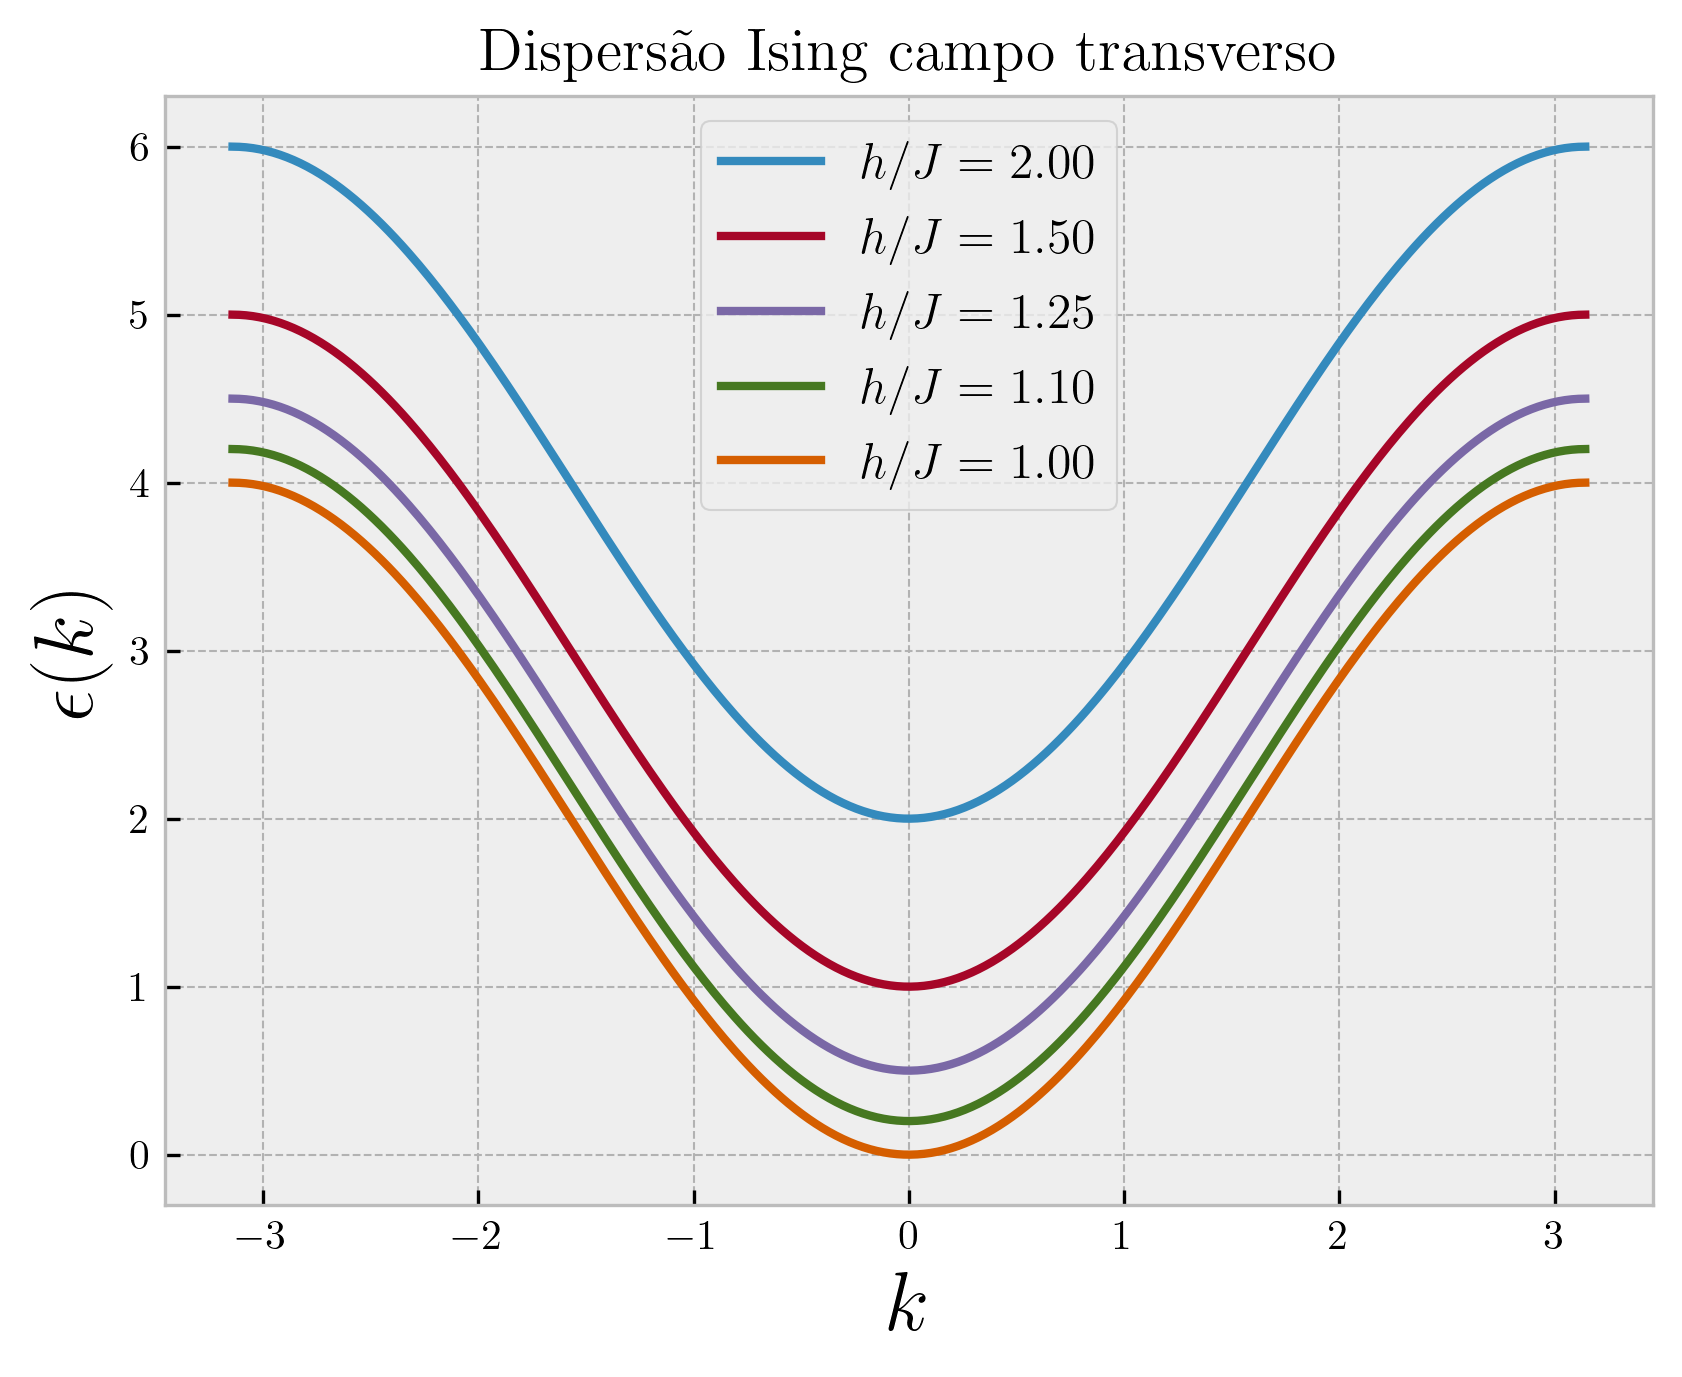
\includegraphics[width=0.5\textwidth]{fig/transv_ising.png}
\caption{Dispersão $\omega(k) = 2\sqrt{J^2 + h^2 - 2hJ \cos k}$ para várias razões $h/J$. Vemos que para $h/J = 1$ a curva forma um cone (fecha o gap).}
\label{fig:transv_ising}
\end{figure}

Olhando para a Figura \ref{fig:transv_ising}, podemos identificar que a transição de fase quântica ocorre quando $h/J = 1$, que é o valor em que a dispersão forma um cone em torno de $k = 0$ (fechamento do gap).

\n

A magnetização é dada por
$$
m_z = \frac{1}{N} \sum_{j} \ev{\s_j^z} = 2 \frac{1}{N}\sum_{k} \ev{f_k^\d f_k} - 1.
$$

Pela transformação de Bogoliubov tem-se
$$
f_k^\d f_k = \cos[2](\theta_k) a_k^\d a_k + \sin[2](\theta_k) a_{-k}a_{-k}^\d
+ i \sin\theta_k \cos\theta_k (a_{k}^\d a_{-k}^\d - a_{-k} a_{-k})
$$

Para $T = 0$ temos que $\ev{X} = \ev{X}{0}$ e que $a_k \ket{0} = 0$. Portanto $\ev{f_k^\d f_k} = \sin[2](\theta_k)$. Usando que $2 \sin[2](x) = \frac{\tan[2](2x)}{1 + \tan[2](2x)}$, obtemos que
$$
m_z + 1 = \int_{-\pi}^{\pi} \frac{J^2 \sin[2](k)}{[h-J\cos(k)]^2 + J^2\sin[2](k)} \dd{k}.
$$
Pedindo para o Mathematica resolver a integral acima, ele retorna
$$
m_z + 1 =
\begin{cases}
\; \pi \frac{J^2}{h^2} , \quad h/J \geq 1, \\
\; \pi , \quad \quad \, h/J < 1. \\
\end{cases}
$$

Acho que o resultado acima não faz sentido né... Mas não sei como consertar.

\n

(d) O hamiltoniano de Kitaev é
$$
H = -t \sum_{i} (f_{i+1}^\d f_i + \hc) - \mu \sum_{i} f_i^\d f_i
+ \Delta \sum_{i} (f_{i+1}^\d f_i^\d + \hc).
$$

É fácil ver que a hamiltoniana do Ising transverso \ref{eq:hamil_transvising} é um caso particular do Kitaev para $\Delta = -J$, $t = J$ e $\mu = -2h$. Como podemos ver em \url{https://topocondmat.org/w1_topointro/1D.html}, para o modelo de Kitaev, a fase trivial acontece para $\abs{\mu} < 2t$ e a topológica para $\abs{\mu} > 2t$. Essas duas fases correspondem à paramagnética e ferromagnética do Ising transversal, respectivamente.

\n\n

\section*{2) Mapa clássico quântico}




%%-----
%% Referências bibliográficas
%%-----
\addcontentsline{toc}{chapter}{\bibname}
%\bibliographystyle{abntex2-num}
\bibliography{citations}
\bibliographystyle{ieeetr}


\end{document}
